%%%%%%%%%%%%%%%%%%%%%%%%%%%%%%%%%%%%%%%%%%%%%%%%%%%%%%%%%%%%%%%%%%%%%%
% amspaper.tex --  LaTeX2e-based template for submissions to American 
% Meteorological Society Journals, including
%
% JAS 	-- Journal of the Atmospheric Sciences
% JAMC 	-- Journal of Applied Meteorology and Climatology
% JPO 	-- Journal of Physical Oceanography
% MWR 	-- Monthly Weather Review
% JTECH -- Journal of Atmospheric and Oceanic Technology
% WAF 	-- Weather and Forecasting
% JCLI 	-- Journal of Climate
% JHM 	-- Journal of Hydrometeorology
% JAM 	-- Journal of Applied Meteorology
%
% Template developed by B. Papa and S. Cooley, AMS. 
% Email questions to latex@ametsoc.org.
%
% August 12, 2008 (SRC)
%	- Clarified/added header notes, comments throughout
%	- Improved title page
%	- Edited text of document for clarity
%	- Altered list styles to adhere to AMS style, added comments
%	- Removed incorrect commands (i.e., \catcode) (corrects umlaut bug)
%	- Moved non-template commands to ametsoc.sty
%
% August, 2008 - B. Papa
% - Updated to handle two column journal page output
% - Updated text with new/modified instructions
%
%%%%%%%%%%%%%%%%%%%%%%%%%%%%%%%%%%%%%%%%%%%%%%%%%%%%%%%%%%%%%%%%     
%%%%%%%%%%%%%%%%%%%%%%%%%%%%%%%%%%%%%%%%%%%%%%%%%%%%%%%%%%%%%%%%
%																															 %
%				USE THIS TEMPLATE, AMETSOC.STY, AND AMETSOC.BST				 %
%			        OR YOUR TEX FILES WILL NOT BE USED				  		 %
%																															 % 
%%%%%%%%%%%%%%%%%%%%%%%%%%%%%%%%%%%%%%%%%%%%%%%%%%%%%%%%%%%%%%%%
%%%%%%%%%%%%%%%%%%%%%%%%%%%%%%%%%%%%%%%%%%%%%%%%%%%%%%%%%%%%%%%%

%%%%%%%%%%%%%%%%%%%%%%%%%%%%%%%%%%%%%%%%%%%%%%%%%%%%%%%%%%%%%%%%%%%%%
% PREAMBLE
%%%%%%%%%%%%%%%%%%%%%%%%%%%%%%%%%%%%%%%%%%%%%%%%%%%%%%%%%%%%%%%%%%%%%
%
% The following two commands will generate a PDF that follows all the requirements for submission
% and peer review.  Uncomment these commands to generate this output (and comment out the two lines below.)
%
% DOUBLE SPACE VERSION FOR SUBMISSION TO THE AMS
\documentclass[12pt]{article}
\usepackage{ametsoc}
%
% The following two commands will generate a single space, double column paper that closely
% matches an AMS journal page.  Uncomment these commands to generate this output (and comment
% out the two lines above. FOR AUTHOR USE ONLY. PAPERS SUBMITTED IN THIS FORMAT WILL BE RETURNED
% TO THE AUTHOR for submission with the correct formatting.
%
% TWO COLUMN JOURNAL PAGE LAYOUT FOR AUTHOR USE ONLY
%\documentclass[10pt]{article}
%\usepackage{ametsoc2col}
\usepackage{subfigure}
\usepackage{comment}
%
%%%%%%%%%%%%%%%%%%%%%%%%%%%%%%%%%%%%%%%%%%%%%%%%%%%%%%%%%%%%%%%%%%%%%
% ABSTRACT
%
% Enter your Abstract here
%%%%%%%%%%%%%%%%%%%%%%%%%%%%%%%%%%%%%%%%%%%%%%%%%%%%%%%%%%%%%%%%%%%%%
\newcommand{\myabstract}{The Weather Research and Forecasting (WRF) model-based variational data assimilation system (WRF-Var) has been extended from three- to four-dimensional variational data assimilation (WRF 4D-Var) to meet the increasing demand for improving initial model states in multi-scale numerical simulations and forecasts. The formulation and preliminary results of WRF 4D-Var had been described in a predecessor paper. 

This article presents the implementation and preliminary results of lateral boundaries control in WRF 4D-Var system. In addition to the initial condition, the lateral boundary conditions are also controlled during the minimization to take into account the impact of observations close to the lateral boundaries. Considering the control of the lateral boundary conditions in 4D-Var is particularly important for assimilating phenomena close to inflow boundary that are well observed during the later part of the assimilation window. Furthermore, To improve the short-range forecast of WRF and reduce the model spin-up time, the precipitation assimilation capability is developed. The NCEP stage IV radar and rain gauge data is able to be assimilated in WRF 4D-Var system. The practical ability to assimilate precipitation data is presented with one heavy rain case and impact of the rainfall data to improve the short-range precipitation prediction is encouraging. The conclusion of assimilating 6h accumulated rainfall data and using of multiple out loops is confirmed by previous studies.

The upgraded features of the new version of WRF 4D-Var presented in this paper is introduced. Firstly, the new WRF 4D-Var is a single program multiple data (SPMD) parallel system, other than a multiple program multiple data (MPMD) system introduced in predecessor paper. The computational efficiency is improved dramatically as a result of the coupling via memory. As a preparation of the operational run of WRF 4D-Var, to reduce the computational cost of 4D-Var run, the multiple-incremental 4D-Var configuration is developed to allow the innovation to be calculated on high resolution during out loop and the inner loop minimization is computed on lower resolution. The  The performance comparison of a ten-day regression analysis/forecast cycles shows that the verification scores from the multiple-incremental 4D-Var run are comparable with the full-resolution 4D-Var run.
}
%
\begin{document}
%
%%%%%%%%%%%%%%%%%%%%%%%%%%%%%%%%%%%%%%%%%%%%%%%%%%%%%%%%%%%%%%%%%%%%%
% TITLE
%
% Enter your TITLE here
%%%%%%%%%%%%%%%%%%%%%%%%%%%%%%%%%%%%%%%%%%%%%%%%%%%%%%%%%%%%%%%%%%%%%
\title{\textbf{\large{Four-Dimensional Variational Data Assimilation for WRF: lateral Boundary Conditions Control,  Precipitation Assimilation and Computational Efficiency Improvements}}}
%
% Author names, with corresponding author information. 
% [Update and move the \thanks{...} block as appropriate.]
%
\author{\textsc{Xin Zhang}
				\thanks{\textit{Corresponding author address:} 
				Dr. Xin Zhang, NCAR/MMM, P.O. Box 3000, 
				 Boulder, CO 80307. 
				\newline{E-mail: xinzhang@ucar.edu}}\\
\textit{\footnotesize{National Center for Atmospheric Research, Boulder, Colorado 80307}}
\and
\centerline{\textsc{Xiang-Yu Huang}}\\% Add additional authors, different institution
\centerline{\textit{\footnotesize{National Center for Atmospheric Research, Boulder, Colorado 80307}}}
}
%
% The following block of code will handle the formatting of the title page depending on whether
% we are formatting a double column (dc) author draft or a single column paper for submission.
% AUTHORS SHOULD SKIP OVER THIS... There is nothing to do in this section of code.
\ifthenelse{\boolean{dc}}
{
\twocolumn[
\begin{@twocolumnfalse}
\amstitle

% Start Abstract (Enter your Abstract above.  Do not enter any text here)
\begin{center}
\begin{minipage}{13.0cm}
\begin{abstract}
	\myabstract
	\newline
	\begin{center}
		\rule{38mm}{0.2mm}
	\end{center}
\end{abstract}
\end{minipage}
\end{center}
\end{@twocolumnfalse}
]
}
{
\amstitle
\begin{abstract}
\myabstract
\end{abstract}
\newpage
}
%%%%%%%%%%%%%%%%%%%%%%%%%%%%%%%%%%%%%%%%%%%%%%%%%%%%%%%%%%%%%%%%%%%%%
% MAIN BODY OF PAPER
%%%%%%%%%%%%%%%%%%%%%%%%%%%%%%%%%%%%%%%%%%%%%%%%%%%%%%%%%%%%%%%%%%%%%
%
\section{Introduction}
The four-dimensional variational data assimilation (4D-Var) technique (Le Dimet and Talagrand 1986; Lewis and Derber 1985) has been pursued actively by the research community and operational centers over the past two decades. The first successful operational 4D-Var system was implemented at the European Centre for Medium-Range Weather Forecasts (ECMWF) using an incremental formulation (Courtier et al. 1994; Rabier et al. 1997). The results demonstrate a significant positive impact on operational forecasts compared to its 3D-Var system (Rabier et al. 2000). Following ECMWF, several operational centers implemented 4D-Var in their operational applications, including Meteo-France (Gauthier and Thepaut 2001), the Met Office (Lorenc and Rawlins 2005; Rawlins et al. 2007), the Japan Meteorological Agency (Honda et al. 2005), and Environment Canada (Gauthier et al. 2007). Other operational centers are also preparing 4D-Var as their data assimilation package, including the High-Resolution Limited-Area Model community (HIRLAM; Huang et al. 2002) and the Naval Research Laboratory Atmospheric Variational Data Assimilation System (NAVDAS-AR; Xu et al. 2005).

The success of the global 4D-Var system in improving global forecasts provided enough encouragement to go ahead with a regional 4D-Var for mesocale and thunderstorm scales. Several regional 4D-Var research systems have been developed, including 1) one based on the fifth-generation Pennsylvania State University National Center for Atmospheric Research (PSU� NCAR) Mesoscale Model (MM5; Zou et al. 1995, 1997; Ruggiero et al. 2006), 2) one based on the National Centers for Environmental Prediction (NCEP) Eta Model (Zupanski 1993), 3) the 4D-Var-based Regional Atmospheric Modeling System (RAMS) data assimilation system (RAMDAS; Zupanski et al. 2005), and 4) the variational Doppler Radar assimilation system (VDRAS) for convective-scale assimilation of radar data (Sun and Crook 1997); 5) the Japan Meteorological Agency (JMA) 4D-Var system (Meso-4DVAR; Koizumi et al. 2005) and NHM-4DVAR (\cite{Kawa2007}), 6) a 4D-Var system for the High Resolution Limited Area Model (HIRLAM) forecasting system (\cite{Gustafd2011}), 7) a 4D-Var system for the Weather Research and Forecasting model (WRF) (\cite{Huang2009}).

The Limited Area Model (LAM) or regional forecasting problem is a lateral boundary condition problem in addition to the initial condition problem. For 
numerical weather prediction, the lateral boundary conditions are generally provided by a host model, for example a global numerical weather prediction 
model. There is much evidence that, for some widely used combinations of domain size and forecast period, forecasts are more sensitive to the LBC specification than to the initial condition (IC) specification within the model domain (Vukicevic and Errico, 1990). This is to be expected because as time advances, features are advected from inflow boundaries into the interior and interior features exit at the outflow boundaries. For regional 4D-Var , the cost function is a function of the initial condition and the lateral boundary condition. 
\begin{comment}
As a starting point, one may that the available boundary conditions from the host model have to be accepted (without change) for usage in the LAM. However, one may use the observations close to the lateral boundaries and let these influence the initial conditions. In case the initial conditions are used as the lateral boundary conditions at the initial time, the subsequent forecast will also be influenced by these observations. Depending on the frequency of the 
updating of the lateral boundary conditions, the host model will gradually take over the definition of the lateral boundary conditions.
\end{comment}

For the control of the lateral boundary conditions in a LAM 4D-Var data assimilation, the tangent linear and adjoint versions of the schemes for the coupling to the larger scale model providing the lateral boundary conditions are needed. \cite{Errico1993} applied the adjoint of the model and its LBC formulation in a limited area model to investigate the sensitivity of limited area model forecast errors to initial as well as lateral boundary conditions. Their research suggested that sensitivity with respect to LBC increases sharply at the time a feature of significant IC sensitivity impacts with the LBC region, and the IC sensitivity may decrease sharply although not disappear entirely.  They also pointed out that the time at which sensitivity with respect to a LBC field has greater magnitude than for a corresponding IC field will be later for a winter case than for a summer case.  A similar study was carried out by \cite{Gusta1998} for a significant storm development over the North Atlantic, indicating that errors in initial as well as in lateral boundary conditions may explain some forecast failures and the sensitivity experiments with respect to the lateral boundary conditions indicate that poor quality lateral boundary conditions may be improved by utilizing subsequent downstream observations within the model integration area. This result may be directly applied in 4D-Var and during the assimilation period the boundary values can be modified together with modifications in the initial state.

With application of 4D-Var for the LAM forecasting, one may control the lateral boundary conditions during the period of the data assimilation window. This may be particularly important for assimilation of phenomena that are observed well inside the LAM domain during the later part of the data assimilation window, while being propagated through the lateral boundaries during the early part of the data assimilation window. If we do not control the lateral boundary conditions, observed information related to these phenomena may be lost. For the control of the lateral boundary conditions in 4D-Var, in the Japan Meteorological Agency (JMA) mesoscale LAM 4D-Var, \cite{Kawa2007} introduced a full model state control variable for the lateral boundary conditions at the end of the assimilation window and a 4D-Var cost function constraint for this new lateral boundary control variable, with a similar form as for the background error constraint. \cite{Gusta2011} follows the JMA approach to control LBC in the HIRLAM 4D-Var and gets a positive impact on a winter storm case over the Scandinavia peninsula in Europe. In WRF 4D-Var, we also follow the JMA approach and we introduce a full model state control variable at the end of assimilation window for the lateral boundary control. The perturbations of model control variables at the start and the end of the assimilation window will be used to estimate the perturbations of the model variable lateral boundary tendencies. 

Assimilation of precipitation has been intensively studied in recent year in an effort to minimize the spin-up/spin-down problems and to provide accurate mesoscale initial states (Park and Zupanski, 2003). A number of studies have been published to demonstrate the potential of 4D-Var for the assimilation of precipitation (Zupanski and Mesinger 1995; Zou and Kuo 1996; Tsuyuki 1996a,b, 1997; Guo et al. 2000; Xiao et al. 2000; Zupanski et al. 2002a,b). D. Zupanski and Mesinger (1995) were the first to assimilate precipitation observations using four-dimensional variational data assimilation approach. They demonstrated the technical feasibility of the approach and showed an improvement of precipitation forecast in mid-latitudes by using a regional NMC eta forecast model and an incomplete adjoint model. Zou and Kuo (1996) indicated the ability of 4D-Var assimilation of precipitation in capturing the detailed structure of mesoscale features by improving the initial conditions, which was crucial for the forecast of MCSs in their case and for reducing the spin-up time. Tsuyuki (1996a,b, 1997) investigated the performance of the 4D-Var technique in the Tropics by assimilating satellite-derived precipitation rates. Not only many feasibility studies of assimilating precipitation data using 4D-Var method published in the literature, but also some operational weather services incorporated precipitation observations operationally, including NCEP, ECWMF, and JMA. It is an impending/urgent issue to incorporate precipitation observations to WRF 4D-Var with the aim of producing more realistic initial atmospheric states and of improving short-range rainfall prediction. 

The assimilation of precipitation observation is potentially very different than that of more conventional observation types for a variety of fundamental and practical considerations (Errico, 2007). In order to use precipitation data in 4D-Var, it is necessary to include parameterization schemes of moist processes into tangent linear model (hereafter TLM) and corresponding adjoint model (hereafter ADM). However these processes are strongly nonlinear and contain discontinuous (non-differentiable) on/off switches, especially in the case of a cumulus convection parameterization. This makes that the tangent linear approximation is less valid for a linearized model with physics than for the same model without physics (Tsuyuki, 1997). Thus, development of the techniques of the 4D-Var data assimilation with realistic, "full-physics" forecast models must be related to examining and solving these problems first (Zupanski and Mesinger 1995), and it may be extremely difficult to keep the right balance between eliminating all discontinuities from complex full-physics forecast model and, at the same time, preserving both the quality of the forecast and efficiency of the code.

Recently, we re-developed the WRF tangent-linear model and adjoint model (hereafter WRFPLUS) based on the latest repository WRF (\cite{Zhangxin2012}). Compared to the previous version of the WRF tangent linear and adjoint models (WAMS) in \cite{Xiao2008}, the performance of WRFPLUS has been dramatically improved compared to the WAMS. The WRF 4D-Var system described in \cite{Huang2009} is a multiple program multiple data (MPMD) system with loose coupling of three components including WRFDA, WRF and WAMS. The information to be communicated among the components is written in and read from disk files. It is very inefficiency on modern distributed memory high performance computers. Furthermore, due to the nature of the sequential iterative algorithm in variational approach, the MPMD framework of the 4D-Var system uses only a subset of the total processors at any moments. Leveraging the development of WRFPLUS, the software design of the WRF 4D-Var has been re-visited and the WRFDA is coupled with WRFPLUS seamlessly into a single program multiple data (SPMD) system. The current work presents a significant improvement on computational efficiency. 

To reduce the computational cost of 4D-Var, a common strategy adopted in operational 4D-Var configuration is the multi-incremental 4D-Var. The key point of this strategy is to calculate innovations on high-resolution nonlinear forward run for out loops and compute the minimization on lower resolution for inner loop. Different out loop may has different resolution. To prepare the feasibility of the operational WRF 4D-Var run, the capability of multi-incremental strategy is also developed and the preliminary experiment results will be demonstrated to confirm the feasibility.

This article is organized as follows. The implementation and impact of the LBC control in the WRF 4D-Var system is put forward in section 2.  Section 3 provides the developments and some preliminary results of assimilation of NCEP stage IV radar and gauge precipitation data. Section 4 includes the works to improve the computational efficiency of WRF 4D-Var, which includes the new development of SPMD WRF 4D-Var and the multi-incremental WRF 4D-Var strategy. The summary and further research perspectives are in section 5.

\section{Lateral boundary conditions control}
\label{sec:lbc}

\subsection{Minimization algorithm}
The WRF 4D-Var algorithm takes the incremental 4D-Var formulation that is commonly used in operational systems (Courtier et al. 1994; Veerse and Thepaut 1998; Lorenc 2003). The incremental approach is designed to find the analysis increment that minimizes a cost function defined as a function of the analysis increment instead of the analysis itself. In the incremental 4D-Var, the tangent linear and adjoint models usually derived from a simplified forward model are used in the inner-loop minimization, while the evolution of the background is predicted with the full forward model. The current WRF 4D-Var system makes use of the following components of the previously developed WRF-Var system (Barker et al. 2005): 1) observation operators, 2) quality control, 3) the background error covariance model. The new developments specified for the current WRF 4D-Var system are : 1) a minimization inner-loop using newly developed simplified WRF tangent linear and adjoint models which will be briefly described later, and 2) an iterative outer loop using the nonlinear WRF model to update the basic trajectory state to account for the effect of nonlinearities in the assimilation algorithm.

The basic WRF 4D-Var system formulation can be found in \cite{Huang2009}. To take into account the constraint of the LBC in minimization, the WRF 4D-Var cost function $J$ turns out to be:
\begin{equation}
J(\mathbf{x}_\mathrm{0},\mathbf{x}_\mathrm{lbc})=J_\mathrm{b}+J_\mathrm{o}+J_\mathrm{c}+J_\mathrm{lbc}
\end{equation}
Compared to the equation (1) in \cite{Huang2009}, in addition to the initial conditions as control variables and basic quadratic measures of distance to the background, observation and balanced solution, the model lateral boundary conditions, $\mathbf{x}_\mathrm{lbc}$ is the new control variable and there is an additional term $J_\mathrm{lbc}$ which measures distance between the analyzed LBC and first guess LBC. It is very important to include the LBC as a control variable since the sensitivity of a forecast aspect with respect to a LBC field has greater magnitude than for a corresponding IC field in winter (\cite{Errico1993}). 

For the control of lateral boundary conditions in WRF 4D-Var, we follow \cite{Kawa2007} 
\begin{equation}
J_\mathrm{lbc}=\frac{1}{2}(\mathbf{x}_\mathrm{lbc}-\mathbf{x}^{\mathrm{b}}_\mathrm{lbc})^T\mathbf{B}^{'-1}(\mathbf{x}_\mathrm{lbc}-\mathbf{x}^{\mathrm{b}}_\mathrm{lbc})
\end{equation}
where $\mathbf{x}_\mathrm{lbc}$ is the lateral boundary condition at the end of the assimilation window, $\mathbf{x}^{\mathrm{b}}_\mathrm{lbc}$ is the first guess of the $\mathbf{x}_\mathrm{lbc}$. $\mathbf{B}^{'-1}$ is the background error covariance matrix for $\mathbf{x}_\mathrm{lbc}$. 


\subsection{Lateral boundary control}
The Limited Area Model (LAM) forecasting problem is not only an initial condition problem but also a lateral boundary condition (LBC) problem. The lateral boundary conditions are generally provided by a host model, for example the forecast of a global numerical weather prediction (NWP) model or a forecast with a larger model domain. The purpose of data assimilation in numerical weather prediction is to combine the real-time and/or past observations with the forecast from a NWP model to produce the analysis, which is considered "the best" estimate of the current state of the system,to be used for the subsequent forecasts. In the four-dimensional variational data assimilation (4D-Var) system of Weather Research and Forecasting (WRF) model, in addition to the control of the initial conditions, the lateral boundary conditions are is also controlled during the minimization to completely take into account the impact of observations close to the lateral boundaries. Considering the control of the lateral boundary conditions in 4D-Var is particularly important for assimilating phenomena close to inflow boundary that are well observed during the later part of the assimilation window. If we do not control the lateral boundary conditions, observed information related to such phenomena may be lost.

For real-data cases, the specified boundary condition is primarily used in WRF and it is also referred to as relaxation or nudging, boundary condition. The specified lateral boundary condition for the coarse grid requires an external file, generated during the same pre-processing for the initial condition file. Let $\mathbf{x}$ be any prognostic model state variable having a lateral boundary entry, following \cite{Davis1977}
\begin{equation}
\frac{\partial{\mathbf{x}}}{\partial{t}}=F_1(\mathbf{x}_\mathrm{lbc}-\mathbf{x})-F_2\Delta^2(\mathbf{x}_\mathrm{lbc}-\mathbf{x})
\end{equation}
where $\Delta^2$ is a 5-point smoothing operator,$ F_1$ and $F_2$ are (nudging) 
weighting coefficients depending on the distance to the lateral boundary, and $\mathbf{x}_\mathrm{lbc}$ is the corresponding boundary value 
provided by the host model. $\mathbf{x}_\mathrm{lbc}$ is specified in the following form:
\begin{equation}
\mathbf{x}_\mathrm{lbc}(t)=\mathbf{x}_\mathrm{lbc}(t_0)+(t-t_0)\frac{\Delta{\mathbf{x}_\mathrm{lbc}}}{\Delta{t}}
\end{equation}
where $\mathbf{x}_\mathrm{lbc}(t_0)$ is the starting point value along the domain boundary relaxation region and $\frac{\Delta\mathbf{x}_\mathrm{lbc}}{\Delta{t}}$ is the corresponding temporal tendency.

For the WRF model, if the LBC update interval is $t_i$ (such as 3h or 6h), then the temporal tendency of $\mathbf{x}$ from $t_{k-1}$ to $t_k$ is calculated as
\begin{equation}
\frac{\Delta{\mathbf{x}_\mathrm{lbc}}}{\Delta{t}}=\frac{\mathbf{x}_\mathrm{lbc}(t_k)-\mathbf{x}_\mathrm{lbc}(t_{k-1})}{t_k-t_{k-1}}
\end{equation}
From equation (3) and (4), we will see that $\mathbf{x}_\mathrm{lbc}(t)$ will depend on $\mathbf{x}_\mathrm{lbc}(t_k)$ and $\mathbf{x}_\mathrm{lbc}(t_{k-1})$, with $t_{k-1}\le{t}\le{t_k}$.

Therefore, considering a data assimilation window from time $t_{k-1}$ until time $t_k$ and it is presently required for WRF 4D-Var that the assimilation window has exactly the same duration as the LBC update interval, we already have $\delta{\mathbf{x}}(t_{k-1})$ ($\delta\mathbf{x}_\mathrm{lbc}(t_{k-1})$) at the start of the window as a assimilation control variable. If we add $\delta{\mathbf{x}}(t_k)$ ($\delta\mathbf{x}_\mathrm{lbc}(t_{k})$) as  another set of assimilation control variables, the quantities needed for the LBC in equation (3) of the tangent linear WRF model are given by
\begin{equation}
\delta{\mathbf{x}}_\mathrm{lbc}(t_{k-1})=\delta{\mathbf{x}}(t_{k-1})
\end{equation}
\begin{equation}
\delta{\mathbf{x}}_\mathrm{lbc}(t_{k})=\delta{\mathbf{x}}(t_{k})
\end{equation}
\begin{equation}
\delta\frac {{\Delta{\mathbf{x}}_\mathrm{lbc}}} {\Delta{t}}=\frac{\delta{\mathbf{x}}_\mathrm{lbc}(t_k)-\delta{\mathbf{x}}_\mathrm{lbc}(t_{k-1})} {t_k-t_{k-1}}
\end{equation}

\begin{comment}
Introduce the lateral boundary condition perturbations as a control variable $\delta{\mathbf{x}_\mathrm{lbc}}(t_k)$  at the end of the data assimilation window (time $t_k$).  For the lateral boundary increment $\delta{\mathbf{x}_\mathrm{lbc}}(t_0)$ at the start of the assimilation window (time $t_0$) we will use the initial condition increment $\delta{\mathbf{x}}(t_0)$. For intermediate time-steps during the integration of the tangent linear model, we will obtain the lateral boundary conditions by the same linear time interpolation scheme that is used in the non-linear model. Once the lateral boundary conditions are defined, the same lateral boundary relaxation scheme, see \cite{Davis1983}, that is used in the non-linear model can also be used in the tangent-linear model, and the adjoint of the lateral 
boundary relaxation is well defined, see \cite{Gusta1998}. Note however, that while the lateral boundary conditions are input data to the tangent linear model, the lateral boundary conditions are output data from the adjoint model. 
\end{comment}

The lateral boundary conditions input to the adjoint model at the end of the assimilation window are $\mathbf{x}_\mathrm{lbc}^\mathrm{ad}(t_k)$ and $(\frac {\Delta{\mathbf{x}}_\mathrm{lbc}} {\Delta{t}})^\mathrm{ad}$
, which will be initialized with zeroes. After the backwards integration of the adjoint model to 
time $t_{k-1}$ the adjoint control variables (or the error gradients) can be obtained 
from: 
\begin{equation}
\mathbf{x}_\mathrm{ic}^\mathrm{ad}(t_{k-1})=\mathbf{x}_\mathrm{ic}^\mathrm{ad}(t_{k-1})+\mathbf{x}_\mathrm{lbc}^\mathrm{ad}(t_{k-1})
\end{equation}
\begin{equation}
\mathbf{x}_\mathrm{ic}^\mathrm{ad}(t_{k-1})=\mathbf{x}_\mathrm{ic}^\mathrm{ad}(t_{k-1})-\frac{1}{t_k-t_{k-1}}(\frac{\Delta{\mathbf{x}_\mathrm{lbc}}}{\Delta{t}})^\mathrm{ad}
\end{equation}
\begin{equation}
\mathbf{x}_\mathrm{lbc}^\mathrm{ad}(t_k)=\frac{1}{t_k-t_{k-1}}(\frac{\Delta{\mathbf{x}_{lbc}}}{\Delta{t}})^\mathrm{ad}
\end{equation}
where $\mathbf{x}_\mathrm{ic}^\mathrm{ad}(t_{k-1})$ denotes the corresponding adjoint model variable of the IC within the relaxation region as provided at the initial time $t_{k-1}$.

Note that $\mathbf{x}_\mathrm{lbc}^\mathrm{ad}(t_{k-1})$ and $(\frac{\Delta{\mathbf{x}_\mathrm{lbc}}}{\Delta{t}})^\mathrm{ad}$ are defined in the boundary relaxtion 
zone only. Consider, however, that they are full domain fields that are 
initialized with zeroes at the end of the data assimilation window and that the boundary relaxation will only fill in values into this full domain 
field inside the boundary relaxation zone.

Also note that the calculation of $J_\mathrm{lbc}$ and $\frac{\partial{J_\mathrm{lbc}}} {\partial{\mathbf{v}_\mathrm{lbc}}}$, where $\mathbf{v}_\mathrm{lbc}$ is the lateral boundary condition control variable in control vector space, will follow exactly the same calculations as for the background error constraint. 

So for practical implementation, the cost function term $J_\mathrm{lbc}$ that quadratically measure the distance to the background LBCs at the end of assimilation window $t_k$ can be written
\begin{equation}
J_\mathrm{lbc}=J(\mathbf{x}(t_k))=\frac{1}{2}\delta{\mathbf{x}}(t_k)^T\bm{\mathbf{B}}_\mathrm{lbc}^{-1}\delta{\mathbf{x}}(t_k)
\end{equation}
where $\bm{\mathbf{B}}_\mathrm{lbc}$ represents the error covariance of the first guess LBCs at the end of the assimilation window. For WRF model, the coarse grid specified lateral boundary is comprised of both a specified and a relaxation zone (see WRF tech note in Fig. 6.1). The specified zone is determined entirely by temporal interpolation from an external forecast or analysis. The width of the specified zone is run-time configurable, but is typically set to 1. The second region of the lateral boundary for the coarse grid is the relaxation zone. The relaxation zone is where the model is nudged or relaxed towards the large-scale forecast. The size of the relaxation zone is also a run-time option and typically set to 4. Apparently, it is very difficulty to calculate and define the physical and statistical relationships in background error covariance just along several rows and columns of the lateral boundary relaxation region. It is practical that we take the whole model states at the end of assimilation window as the control variables and just use the model variables along lateral boundary relaxation region to calculate the lateral boundary conditions. Therefore, the $\bm{\mathbf{B}}_\mathrm{lbc}$ should take the same definition as $\bm{\mathbf{B}}$. As a reasonable assumption, we will apply $\bm{\mathbf{B}}_\mathrm{lbc}=\bm{\mathbf{B}}$ in our experiments. 

One may question whether the assumption of $\bm{\mathbf{B}}_\mathrm{lbc}=\bm{\mathbf{B}}$ is suitable because it is possible that high correlations may exist between the model state control variables at the start and end of the assimilation window. \cite{Gusta2011} takes statistics for vorticity as an example to check the differences between background forecast error statistics and forecast tendency error statistics estimated by NMC method. His estimation shows that the standard deviations for the forecast tendency differences are significantly larger than the standard deviations for full forecast differences in the middle troposphere and that the vorticity forecast differences are only weakly correlated over 5h in time. Therefore, for the 4D-Var with LBC control we may assume that the weak correlation in time of vorticity increments would make the minimization reasonably well conditioned.

\begin{comment}
One potential problem is that the introduction of the lateral boundary 
condition constraint in the form described above, would worsen the conditioning of the 4D-Var minimization problem, since the lateral boundary condition errors at the end of the assimilation window would be strongly 
correlated with the initial condition errors at the start of the assimilation 
window, at least for the large scale and slowly varying phenomena that are 
important for the lateral boundary conditions. One simple pre-conditioning 
would be to subtract the lateral boundary conditions at the start of the 
assimilation window from the lateral boundary conditions at the end of 
the assimilation window, thus to treat the tendency of the lateral boundary 
conditions 
\begin{displaymath}
(\frac{\partial{\delta{\mathbf{x}_\mathrm{lbc}}}}{\partial{t}})=\frac{\delta{\mathbf{x}_\mathrm{lbc}}(t_k)-\delta{\mathbf{x}_\mathrm{lbc}}(t_0)} {t_{k}-t_0}
\end{displaymath}
as the control variable. This approach would also require the covariance of forecast tendency errors, that possibly 
could be estimated by the NMC method from differences between forecast 
tendencies valid at the same time. 
\end{comment}

\subsection{Single observation experiments with LBC control}
\label{sec:single}
Analysis increments due to a single observation produced by a data assimilation system implicitly provide the effective background error covariance matrix $\mathbf{B}$ and describe how the tangent linear and adjoint model propagate the observational information, see \cite{Huang2009}. After any new capability for the WRF 4D-Var system was developed, a single observation experiment is an effective and clean way to show the impact of the new capability on the analysis.

Given a single temperature observation at the end of the time window of 4D-Var, we knew that the 4D-Var increments have a temporal dimension, the increments at 6 h give a graphic representation of the background error covariance matrix at 6 h, $\mathbf{MBM}^T$, where $\mathbf{M}$ and $\mathbf{M}^T$ are the WRF tangent linear model and adjoint model, respectively. For the current regional WRF 4D-Var, both the initial condition and the lateral boundary conditions determine the future trajectory of the model. Therefore, the observations close to or within the lateral boundary relaxation region should not only impact the initial condition but also the lateral boundary condition.

%The first experiment has a single observation at 6 h, which is far from the lateral boundary and the tendency from LBC should have trivial or no impact on the observation location at 6 h, which means assimilating this observation either with or without LBC control should make little/no difference on the analysis at 0 h. The second experiment also has a single observation at 6 h, but close to the lateral boundary and the tendency from LBC should have significant impact on the observation location at 6 h, which means assimilating this observation with or without LBC control should make big difference on the analysis at 0 h.

We still use the same demonstration case as in \cite{Huang2009},  which is a severe winter storm case that occurred at 0000 UTC 25 January 2000. The forecast background valid at 0000UTC 25 January 2000 is produced by a WRF nonlinear model 12h run with full physics from interpolated NCEP final analysis for 1200 UTC 24 Janyary 2000. A pseudo single 500hPa temperature observation at the end of the assimilation window, 0600 UTC, is placed at $28\,^{\circ}\mathrm{N}$, $75\,^{\circ}\mathrm{W}$, the red cross in Fig.~\ref{fig:lbc}. This pseudo observation is a 500hPa temperature of 254K with an assumed error of 1K. We select this location on purpose because there is strong inflow from the southern lateral boundary and the pseudo observation has -0.95K difference with the first guess at the end of the data assimilation window. Since the observation location is around 200km away from the southern lateral boundary and still within the boundary relaxation region, we expect the forward non-linear model and the tangent-linear model to propagate (a part of) observed information from the boundary into the inner domain and the backward adjoint model to propagate the error gradient information from the inner domain back to the boundary condition. If only the initial condition is controlled during the 4D-Var minimization, probably it is difficult for the forecast trajectory from the analysis to fit the observation at the later part of assimilation window. 

Temperature assimilation increments at 500 hPa for the case of controlling lateral boundary condition are show from +0h until +6h into the data assimilation window in Fig.~\ref{fig:lbc}. Because the observation is within the lateral boundary relaxation region, the evolution of the temperature at the observation location during the assimilation window is comprised of two contributions: the first contribution is from the model dynamics and physics and the second contribution is from the nudging effects coming from the southern lateral boundary conditions. Therefore, we can expect the error gradient output from backward adjoint model will influence the initial condition and the lateral boundary condition as well. 

In Fig.~\ref{fig:lbc}, there are very clearly flow-dependent increments created upstream the observation at +00h, it is the analysis response in initial condition to the 6h observation, which is consistent with the expectation described above. During the 4D-Var minimization, the cost function includes an additional term to control the lateral boundary conditions, although it is not that meaningful to show the increments in the boundary condition here,  the boundary conditions at both start and the end of the assimilation window are changed during the minimization. In Fig.~\ref{fig:lbc}, from +00h to +06h ,we notice a smoothly varying assimilation increment that
is slowly moving towards the observation location during the 6 hour data assimilation window, with a maximum increment of approximately -0.48K at +06h in the vicinity of the simulated observation at  $28\,^{\circ}\mathrm{N}$, $75\,^{\circ}\mathrm{W}$. One may argue that this increment evolution is not necessarily only related to the boundary condition, rather than it receives contribution from several model processes in model.

The same single observation impact experiment was repeated, but now without control of the lateral boundary conditions. Fig.~\ref{fig:nolbc} presents the increment evolution without LBC control from +00h to +06h. The interesting thing is the analysis increment at +00h in Fig.~\ref{fig:nolbc} is almost exactly the same with the +00h increment in Fig.~\ref{fig:lbc}, which means that the 4D-Var minimization produces a similar response in the initial condition. However, as the time advances from +00h to +06h, the major increment pass through the observation location. At the end of the assimilation window, the maximum center of the increment is located downstream of the observation and the increment at the observation location is only -0.04K. In this case, the 4D-Var minimization only adjust the initial condition and the boundary condition at the start of the assimilation time window, the boundary condition at the end of the assimilation window will continue to be untouched. A proper assimilation of the simulated observation in this case can only be achieved through control of the lateral boundary conditions at the end of the data assimilation window.

\subsection{Real observation assimilation experiments with and without control of lateral boundary conditions}

\subsubsection{The model and data assimilation setup}
In order to validate the impact of the lateral boundary condition constraint in WRF 4D-Var, experiments with two methods described in section 2 (nolbc and lbc) were carried out for a period of 5 days. The period of December 1999 was selected since this month was characterized by several mesoscale storm developments over Europe. WRF 4D-Var with a single outer loop iteration was applied and the experiments were done for the operational SMHI 11 km HIRLAM domain, see Figure \ref{fig:denmark_domain}, and with 45 vertical levels. The operational SMHI 30 km HIRLAM domain includes 121 x 91 horizontal grid points. This relatively small forecast domain was chosen on purpose in order to maximize the possibilities to find an impact from controlling the lateral boundary conditions. The WRF nonlinear forward model applies the physical parameterizations include the WRF Single-Moment 5-class microphysics scheme, the Mellor-Yamada-Janjic PBL scheme, Noah Land Surface Mode, eta similarity surface layer scheme,  Grell 3D cumulus scheme, RRTM longwave radiation scheme and Goddard shortwave radiation scheme. Lateral boundary conditions were obtained from forecasts available at 00UTC and 12UTC in the ECMWF ERA-40 re-analysis data sets (\cite{Uppala2005}). The WRF 4D-Var used the GTS conventional observational data and was applied with a 6h data assimilation cycle. Forecasts up to +48 h were produced at 00UTC, 06UTC, 12UTC and 18UTC. 

\subsubsection{Forecast verification results}

The forecasts produced by the experiments were verified against ECMWF ERA-40 re-analysis data sets. Forecast root mean square error (RMSE) is presented. All verification scores showed a small positive or a neutral impact of the control of lateral boundary conditions. Scores for verification of relative humidity forecast profiles against ECMWF re-analysis are included in Figure \ref{fig:denmark}. We may notice a positive impact of the scores from the experiment testing the control of lateral boundaries. By looking at the verification scores for forecast of wind, temperature and moisture  (Figure \ref{fig:denmark_24h}) over a European domain we see a clear increase in the RMSE (root mean square error) verification scores at forecast length 24h for the experiments without control of lateral boundaries in comparison with the experiments with control of lateral boundaries. This should be interpreted as a difficulty for the assimilation to adapt to observations close to the lateral boundaries, a similar feature that we already noticed through the single simulated observation experiments. Repeating the verification against ECMWF re-analysis for forecast length 48h, the advantages of experiments with control of lateral boundaries are more obvious. (Figure \ref{fig:denmark_48h}).


\section{Precipitation assimilation}

\subsection{Implementation details of precipitation assimilation in WRF 4D-Var}
Direct four-dimensional variational data assimilation (4D-Var) of NCEP stage IV radar and gauge precipitation observations over the United States has been developed and tested in WRF 4D-Var system. The observations to be assimilated in this study are NCEP stage IV precipitation data, which combine precipitation estimates from about 150 Doppler Next Generation Weather Radar (NEXRAD) with about 5500 hourly rain gauge measurements over the continental United States (Baldwin and Mitchell 1996; Lin and Mitchell 2005). The original precipitation data are available on a 4-km resolution polar-stereographic grid and are thinned onto the 60km resolution. 

In WRF 4D-Var system, the model state consists of temperature, humidity, wind and surface pressure. To assimilate the precipitation observations, simplified paramaterizations of convection (Zhang 2012) and large-scale moist processes (Zhang 2012) are used in tangent linear and adjoint integration for each minimization. Other processes also represented include vertical diffusion, and gravity wave drag (Zhang, 2012).

To better satisfy the requirement of Gaussian distributions of observation errors in 4D-Var and to avoid the sub-optimality of the 4D-Var analysis (Errico et al. 2000), the logarithmic transform, namely $\ln(RR+1)$, is applied to observed and model equivalent precipitation amounts (RR, expressed in mm h21) before the assimilation. Such a transformation was successfully used by Mahfouf et al. (2007) and Lopez (2011). Also, in order to better satisfy the 4D-Var linearity assumption, as discussed in Lopez (2011), it was decided to consider 6-h precipitation accumulations, still expressed in millimeters per hour, instead of the original hourly precipitation data. We did some experiments to assimilate the hourly precipitation data, the the 

As already implemented for all other observation types in 4D-Var, precipitation observations are subjected to an a priori first-guess check, which rejects measurements that depart too much from the model background. In the present case, a precipitation observation is rejected if $|y-H(x_b)|>5\sigma_o$, where $\sigma_o$  is the observation error standard deviation in $\ln(RR+1)$ space and is set equal to 0.18 followed the discussion in Lopez (2011). In other words, all observations leading to absolute values of background departures larger than 1.02 in $\ln(RR6h+1)$ space are screened out. This first-guess check for precipitation data is only applied in the first trajectory of each 4D-Var cycle, as for all other observation types.

\subsection{Experiment design}

Th heavy rain case happen from 06 UTC 8 June 2009 has been selected for running experiments of direct 4D-Var assimilation with NEXRAD precipitation observations over the continental United States domain. This periods was chosen because they were characterized by numerous precipitating events of both convective and stratiform nature. For this period, two 4D-Var experiments were performed: a control run (CTRL) that uses all standard conventional observations available as in NCEP Prepbufr and an experiment (4DVAR) with NCEP Stage IV 6-hourly precipitation accumulations also included in the 4D-Var assimilation process. All experiments were run with 45 vertical levels and with a horizontal resolution of 60 km with 105X72 grid points in the 4D-Var trajectory computations as well as in the subsequent 24h forecasts started from 4D-Var analyses. 

\subsection{Precipitation scores}
Fig. \ref{fig:rainfall} is the simulated and observed 6h precipitation from 06 UTC 8 June 2009 to 12 UTC 8 June 2009, respectively. (Should add TS scores comparison etc)



\section{Coupling of the WRFPLUS and WRFDA into a single executable 4D-Var system}

NCAR started to develop its first version of the tangent linear (hereafter TLM) and adjoint models (hereafter ADM) for the WRF ARW core around 2005 and research based on this version has been conducted and published (\cite{Xiao2008}). The first version of TLM and ADM, as well as WRF nonlinear forward model (hereafter FWM) model were also coupled with WRFDA into a multiple program multiple data (MPMD) WRF 4D-Var system (\cite{Huang2009}). In this MPMD WRF 4D-Var, WRFDA calls WRF FWM, WRF TLM and ADM via system calls. It communicates information among the WRFDA, the WRF FWM, the TLM and the ADM via files. Launching the MPMD version of WRF 4D-Var system consisted of the following steps:
1. Starting a multitask (via MPI) execution of the WRFDA. 2. Starting a multitask (via MPI) execution of the WRF model. 3. Starting a multitask (via MPI) execution of the WRF FWM/ADM. The end of the execution of the WRF 4D-Var model happened when all three executables had finished their tasks or an error condition occurred. During the coupling, exchanges data were written to disk and signal files used by each component to inform the other components that data were ready to be read.

For high resolution modeling which needs to run on modern supercomputers with a distributed memory system, the MPMD 4D-Var system using disk files to communicate information severely limits the number of processors that can be used. Specifically, the basic states trajectory represented by the forecasted atmospheric state at every time steps within the assimilation window has to be saved by FWM and has to be read in during TLM and ADM integration. The costs of the gather and scatter operations across large number of distributed processors are extremely expensive. Another issue is that the $MPI\_COMM\_WORLD$ communicator (defining the global �addresses� of MPI tasks) is split into �private� communicators for the WRFDA model, the WRF FWM and the WRF TLM/ADM, respectively. Due to the sequential iterative algorithm of variational data assimilation, only one component of the coupled system is running at any moment and a subset of processors associated the component are participating the computing, the remain processors are idle, see schematic diagram fig. \ref{fig:coupling_mpmd}. Therefore, a single execution system based on explicit (e.g. via the Message Passing Interface (MPI)) message passing needs to be used. 

The proposed approach to coupling WRFDA, WRF and WRF TLM/ADM is to integrate them into a single program multiple data (SPMD) system . Since WRFDA and WRF TLM/ADM share the same software infrastructures (such as registry, grid definition, parallelization strategy and I/O etc.) with WRF and the regridding is not necessary, it is very natural and easy to let them share a common software framework.  The $MPI\_COMM\_WORLD$ communicator is no longer split into �private� communicators and all components share the the same communicator to ensure that all processors are attending the computation at any time. All MPI communications within the component models is now done via memory copy, see schematic diagram fig. \ref{fig:coupling_spmd}

\subsection{Upgrade to WRFPLUS}

In the past few years, the WRF model and WRFDA system have experienced extensive changes. However, the first version of WRF TLM and ADM has failed to catch up with the changes of the WRF and WRFDA systems and the obsoleted TLM and ADM models is no longer suitable for the development of the SPMD WRF 4D-Var system.

From the WRF model version 3.2 release, we started to re-develop the tangent linear and adjoint models of WRF ARW core based on the latest WRF. Compared to its first version, the new version has following improvements: 1) All-in-one system, the newly developed system includes WRF FWM, the TLM and the ADM under one software framework (hereafter WRFPLUS); 2) Consistent with the latest WRF development, the current tangent linear and adjoint codes are always synchronized with the WRF changes; 3) Significant improved parallel efficiency; 3) Improved physics packages, in addition to vertical diffusion and surface drag, we also include a simplified microphysics scheme and a simplified cumulus scheme (\cite{Zhangxin2012});  4) Accurate and complete procedures for tangent linear and adjoint checks are included to make sure that the existing codes and newly developed codes are error free; 5) A set of coupling interfaces has been developed for coupling with other systems such as the subroutine interfaces of WRF tangent linear and adjoint codes are constructed. For details of WRFPLUS, see \cite{Zhangxin2012}.


\subsection{Performance and scalability of WRF 4D-Var system}

In a coupled system, the overall parallel scalability depends on the individual scalabilities of each components and the cost to communicate the information. The WRFPLUS model is known to scale quite well (\cite{Zhangxin2012}), so we expect that the WRFDA and/or the information communication might be the limiting factor. 

Figure XXX shows the wall clock time (top plot) and speed-up (bottom plot) of the WRF 3D-Var FGAT for 450x450x51L,15km and 6h assimilation window configurations and of WRFDA 3D-Var run for the the same configuration for 5 iterations minimization as function of number of CPU cores. These runs were done on the IBM Power6 machine at bluefire of NCAR. The main difference between the two experiments is that the FGAT run has all the information communication as in 4D-Var, but the TLM and ADM are identity models.

Two things are evident from the figure; the 3D-Var model is .......

Figure 5 shows the wall clock time (top plots) and speed-up (bottom plots) as function of number of CPU cores for two different IFS resolutions. Just like figure 4 these runs were done on the IBM Power6

Figure \ref{performance} show the performance comparison between the single executable WRF 4D-Var and the MPMD WRF 4D-Var with identity WRF TL/AD.  Although this experiment doesn't include the WRF TL/AD realistic running, the significant performance improvement is still achieved due to aforementioned single executable application and memory IO.

Figure \ref{4dvartime} is the performance of a big case ......



\section{Multi-incremental WRF 4D-Var}

The WRF 4D-Var algorithm (\cite{Huang2009}) takes the incremental 4D-Var formulation that is commonly used in operational systems (Courtier et al. 1994; Veers� and Th�- paut 1998; Lorenc 2003). The incremental approach is designed to find the analysis increment that minimizes a cost function defined as a function of the analysis increment instead of the analysis itself. In the incremental 4D-Var, the tangent linear and adjoint models usually derived from a simplified forward model are used in the inner-loop minimization, while the evolution of the background is predicted with the full forward model. This approximate quadratic minimization problem is solved using an iterative algorithm: this is the inner loop of 4D-Var. At the time of this study of WRF 4D-Var, the conjugate gradient algorithm is used to solve the inner loop minimization problem. After this minimization, the departures and trajectory can be recomputed using the non-linear model and a new linearized problem is defined around an improved guess. The process can be repeated: this is the outer loop of incremental 4D-Var. If the linearized problem is reasonably close to the non-linear problem, its solution should be an approximation of the solution of the non-linear problem. At the next outer loop iteration, the starting point is closer to the solution, the quadratic approximation is more accurate and should in principle provide a more accurate solution to the non-linear problem.

In order to reduce the computational cost of the WRF 4D-Var data assimilation process, the inner loop minimizations are run at lower resolution than the forecast. Multiple inner loop minimizations are able to run with different resolutions. An initial experiment of the denmark storm case used in section \ref{sec:lbc} was run to test the performance. The testing platform is a Linux cluster with multiple 2.27GHz Intel\textsuperscript\textregistered Xeon\textsuperscript{\textregistered} X7560 processors. On average, Using 32 processors, the 35 iterations of 4D-Var minimization run with one out loop using consistent horizontal resolutions (both inner and out loops use 30KM horizontal resolution, hereafter full-resolution 4D-Var) takes about 4 hours to finish the analysis. However, with the multi-incremental configuration where the out loop was set to run on 30KM and the minimization of inner loop was set to run on 90KM, the 35 iterations only takes 22 minutes with 16 processors. Specifically, the high resolution innovation calculation part takes about 2 minutes and the lower resolution inner loop minimization takes 20 minutes to complete.

To further valid the impact of the multi-incremental WRF 4D-Var, the denmark case experiment is re-ran for 10 days with the multi-incremental strategy. The comparison of the verification scores for 0h analysis and 24h forecast between the full-resolution 4D-Var and the multi-incremental 4D-Var are presented in figure \ref{fig:multi_inc_0h} and the figure \ref{fig:multi_inc_24h} is for 24h forecast. It is evident that the multi-incremental 4D-Var strategy doesn't impact the analysis and forecast performance too much and all the verification scores from the two experiments are comparable in this experiment. ( needs more discussion on why)


\section{Conclusion}


\begin{figure}[t]
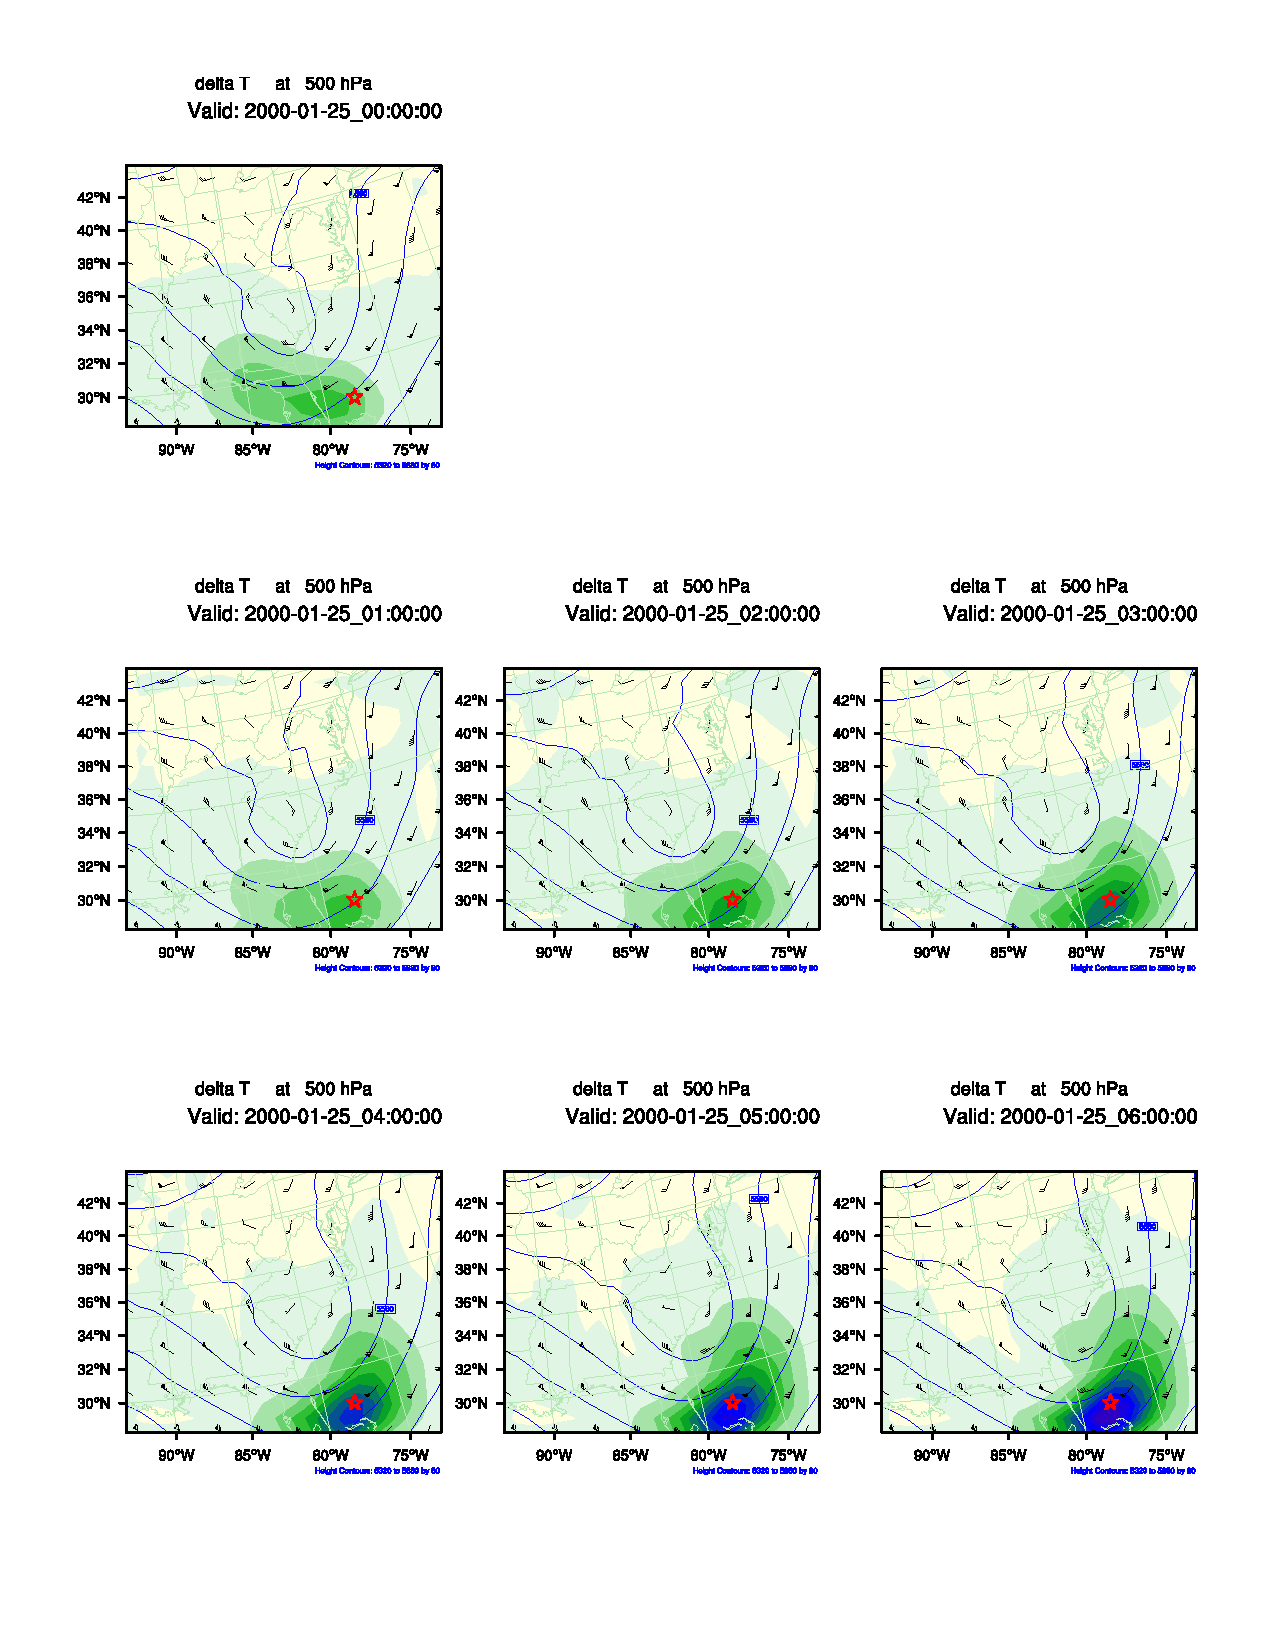
\includegraphics[scale=0.7]{./figures/lbc}
\caption{Evolution of 500hPa potential temperature perturbation with LBC control.}\label{fig:lbc}
\end{figure}

\begin{figure}[t]
\noindent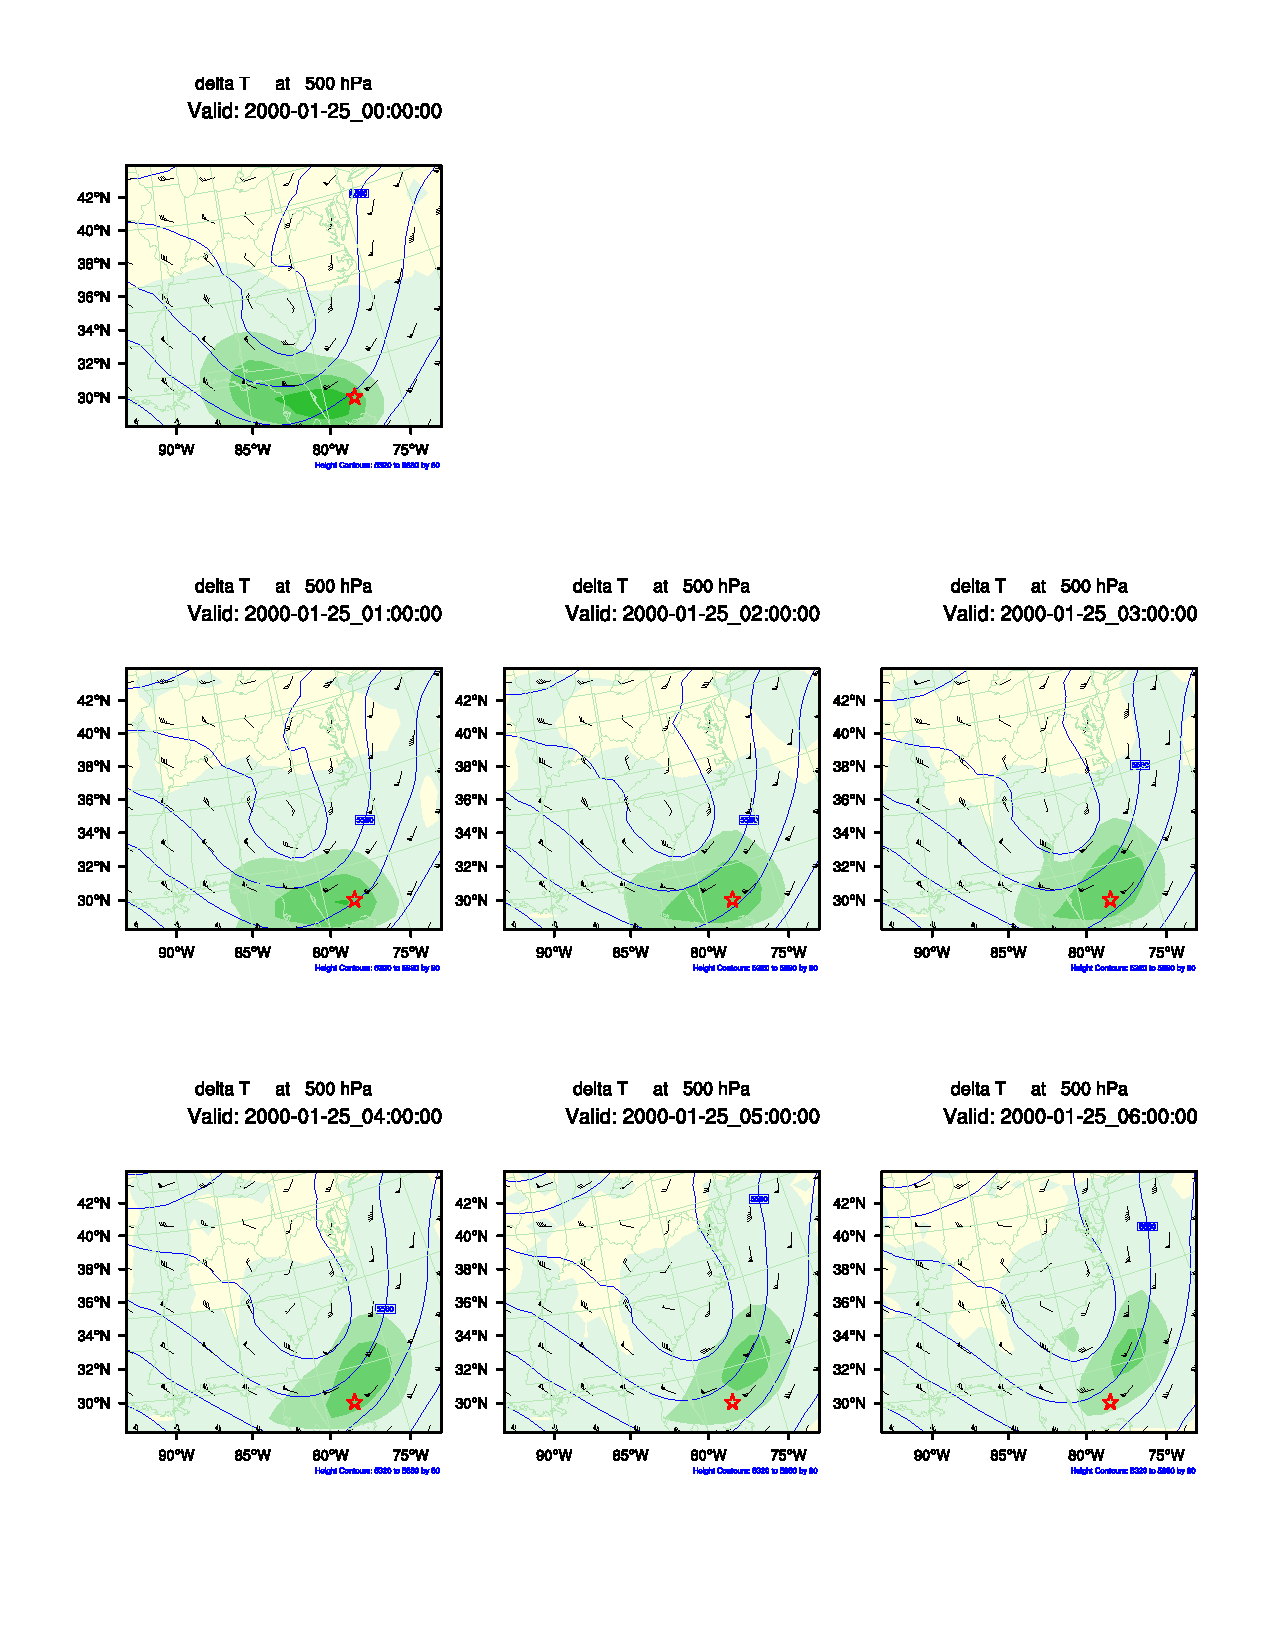
\includegraphics[scale=0.7]{./figures/nolbc}
\caption{Evolution of 500hPa potential temperature perturbation without LBC control.}\label{fig:nolbc}
\end{figure}

\begin{figure}[t]
\noindent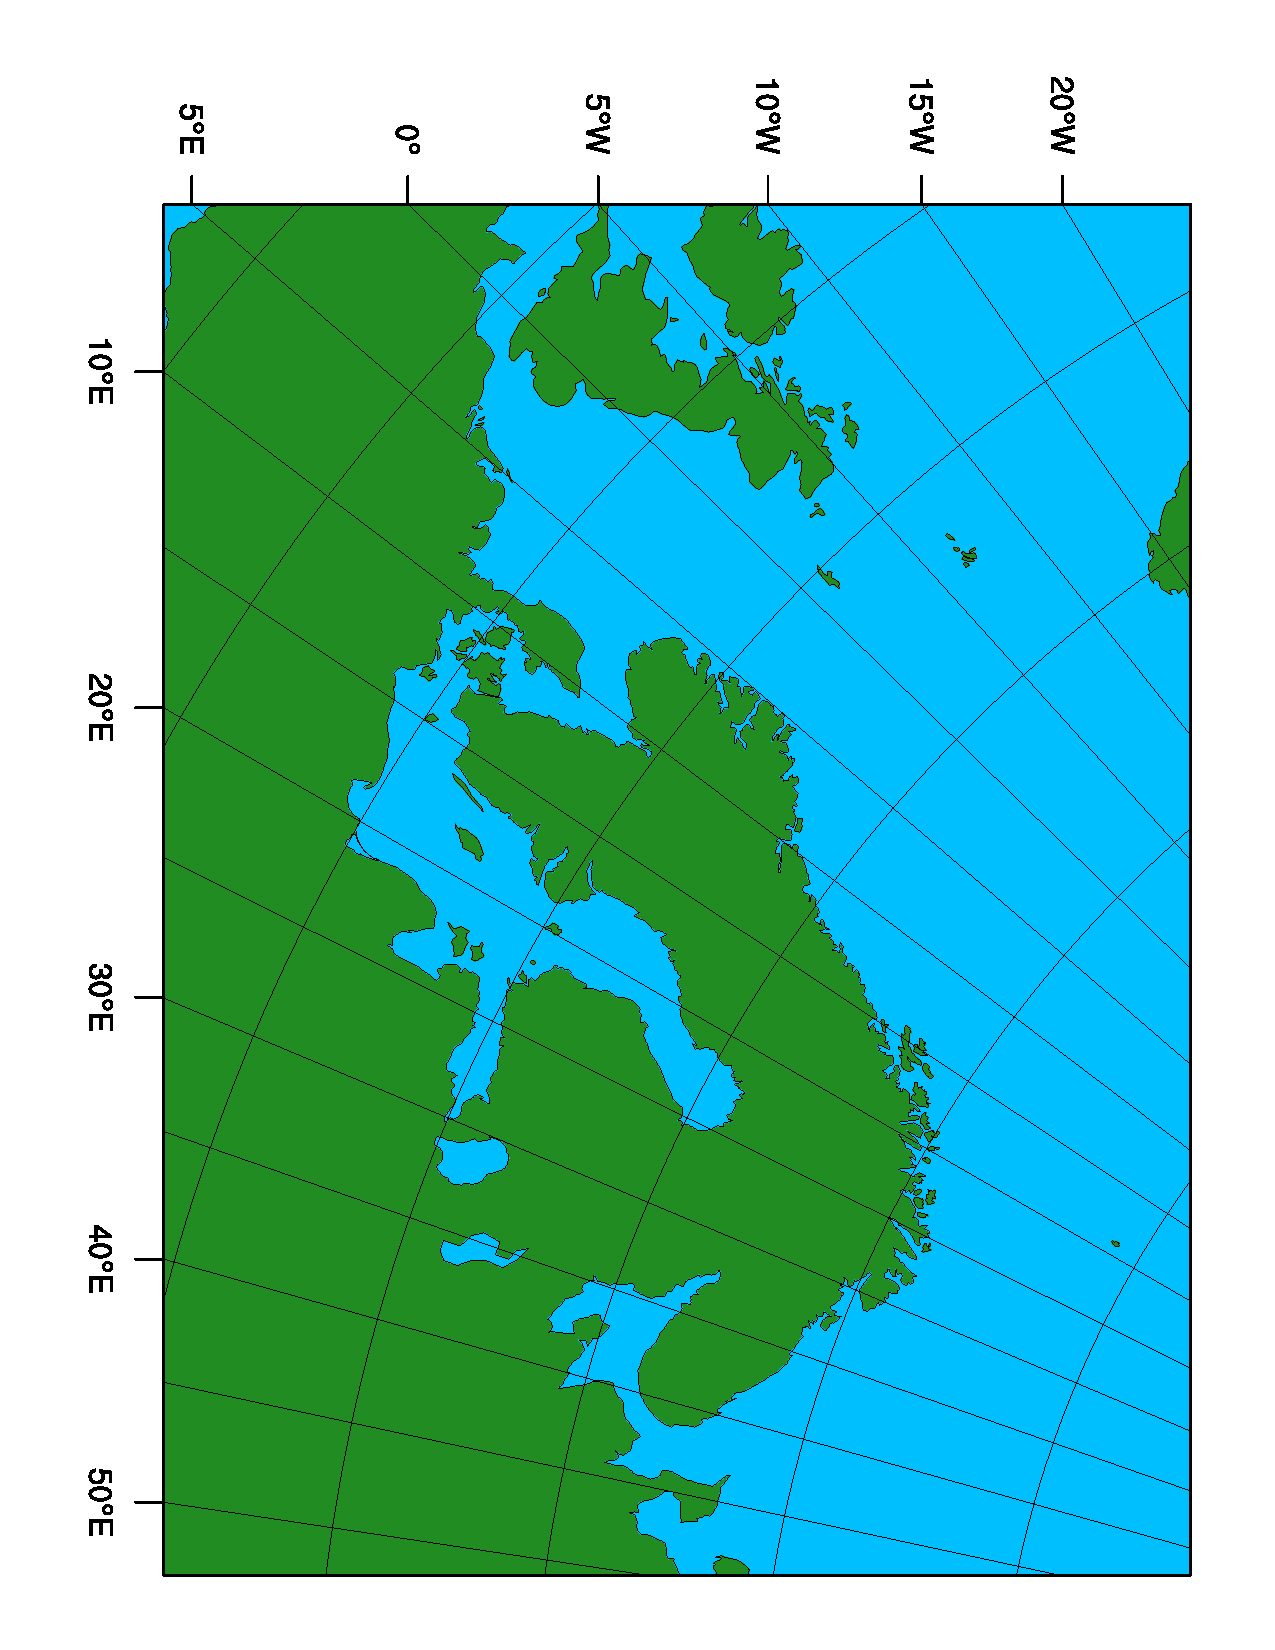
\includegraphics[angle=90, scale=0.6]{./figures/denmark_domain.pdf}
\caption{The Scandinavian case data assimilation and forecast domain.}\label{fig:denmark_domain}
\end{figure}

\begin{figure}[t]
     \begin{center}
%
        \subfigure[Vertical profiles of RMSE for 24h forecast]{%
            \label{fig:denmark_24h}
            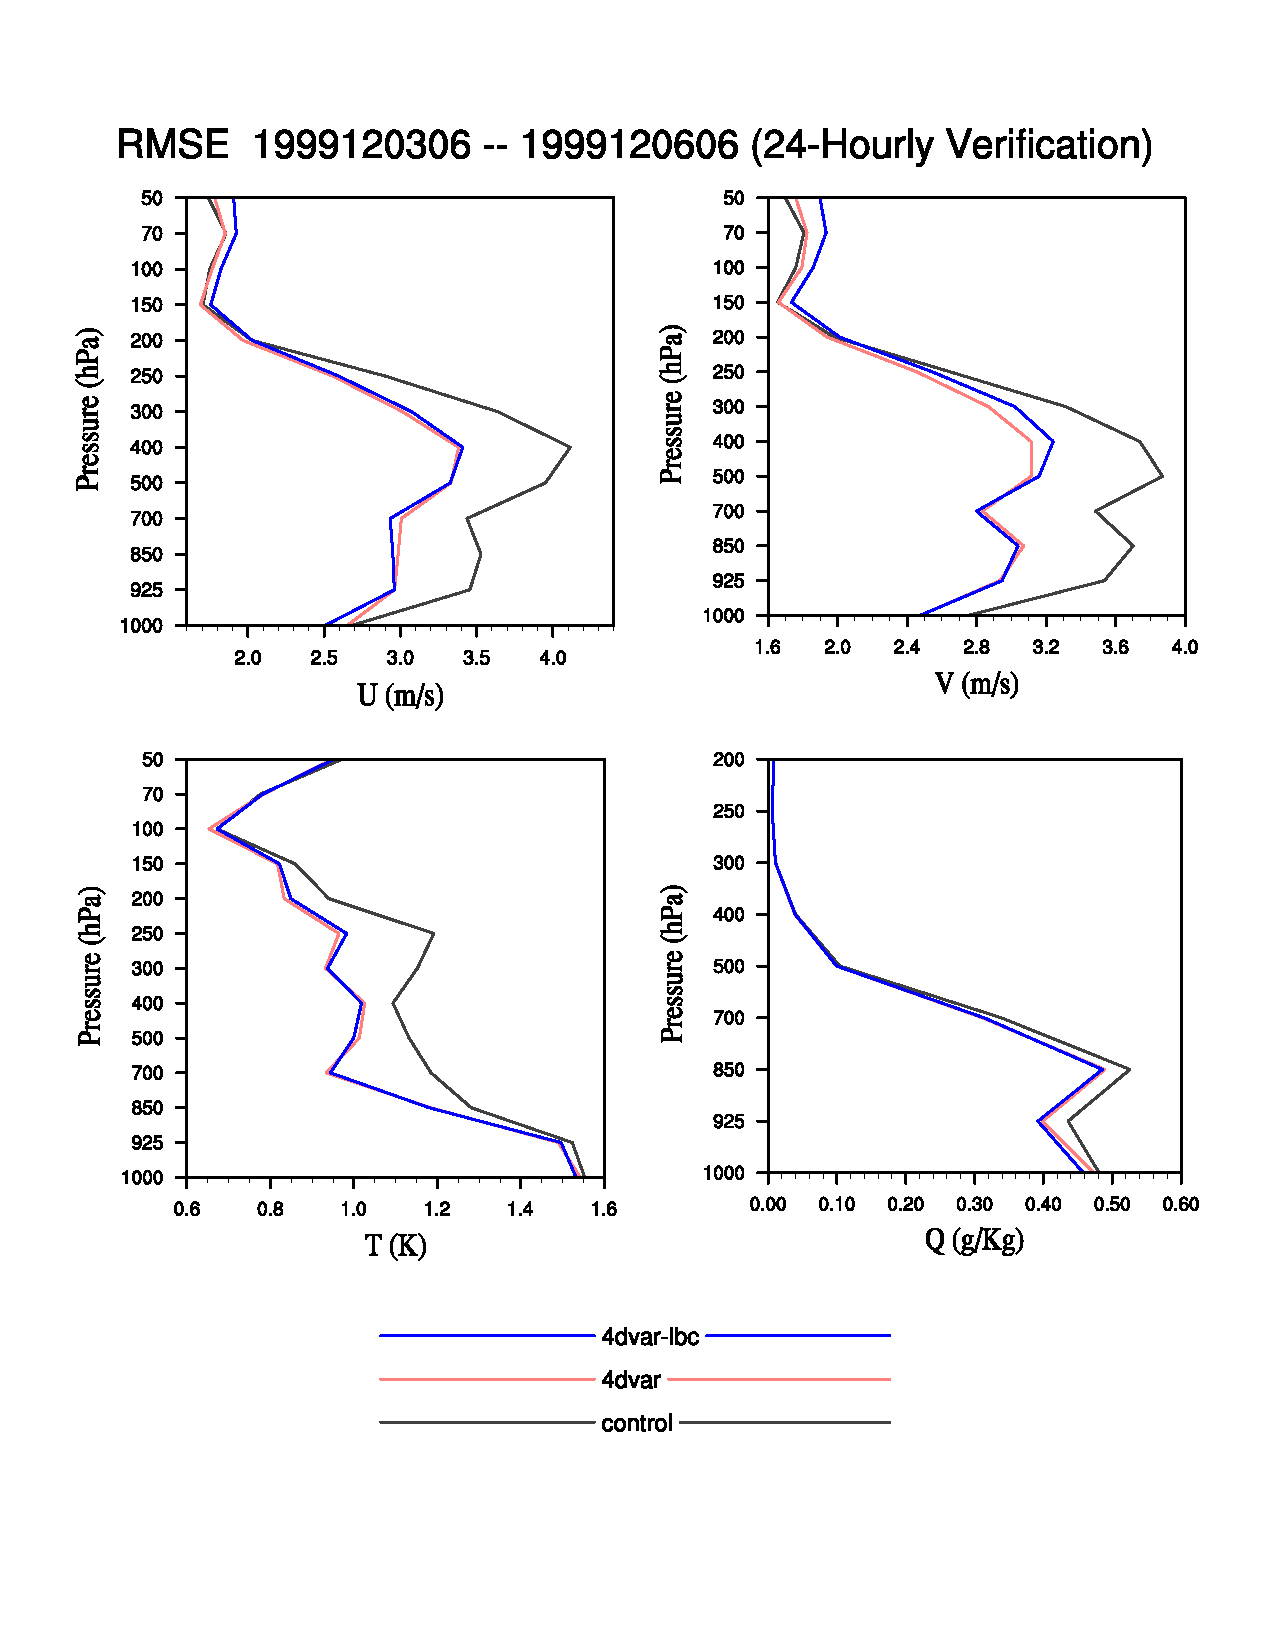
\includegraphics[trim=0cm 6cm 0cm 0cm, clip=true, width=0.5\textwidth]{figures/Profile_RMSE-hr24_lbc.pdf}
        }%
        \\
        \subfigure[Vertical profiles of RMSE for 48h forecast]{%
           \label{fig:denmark_48h}
           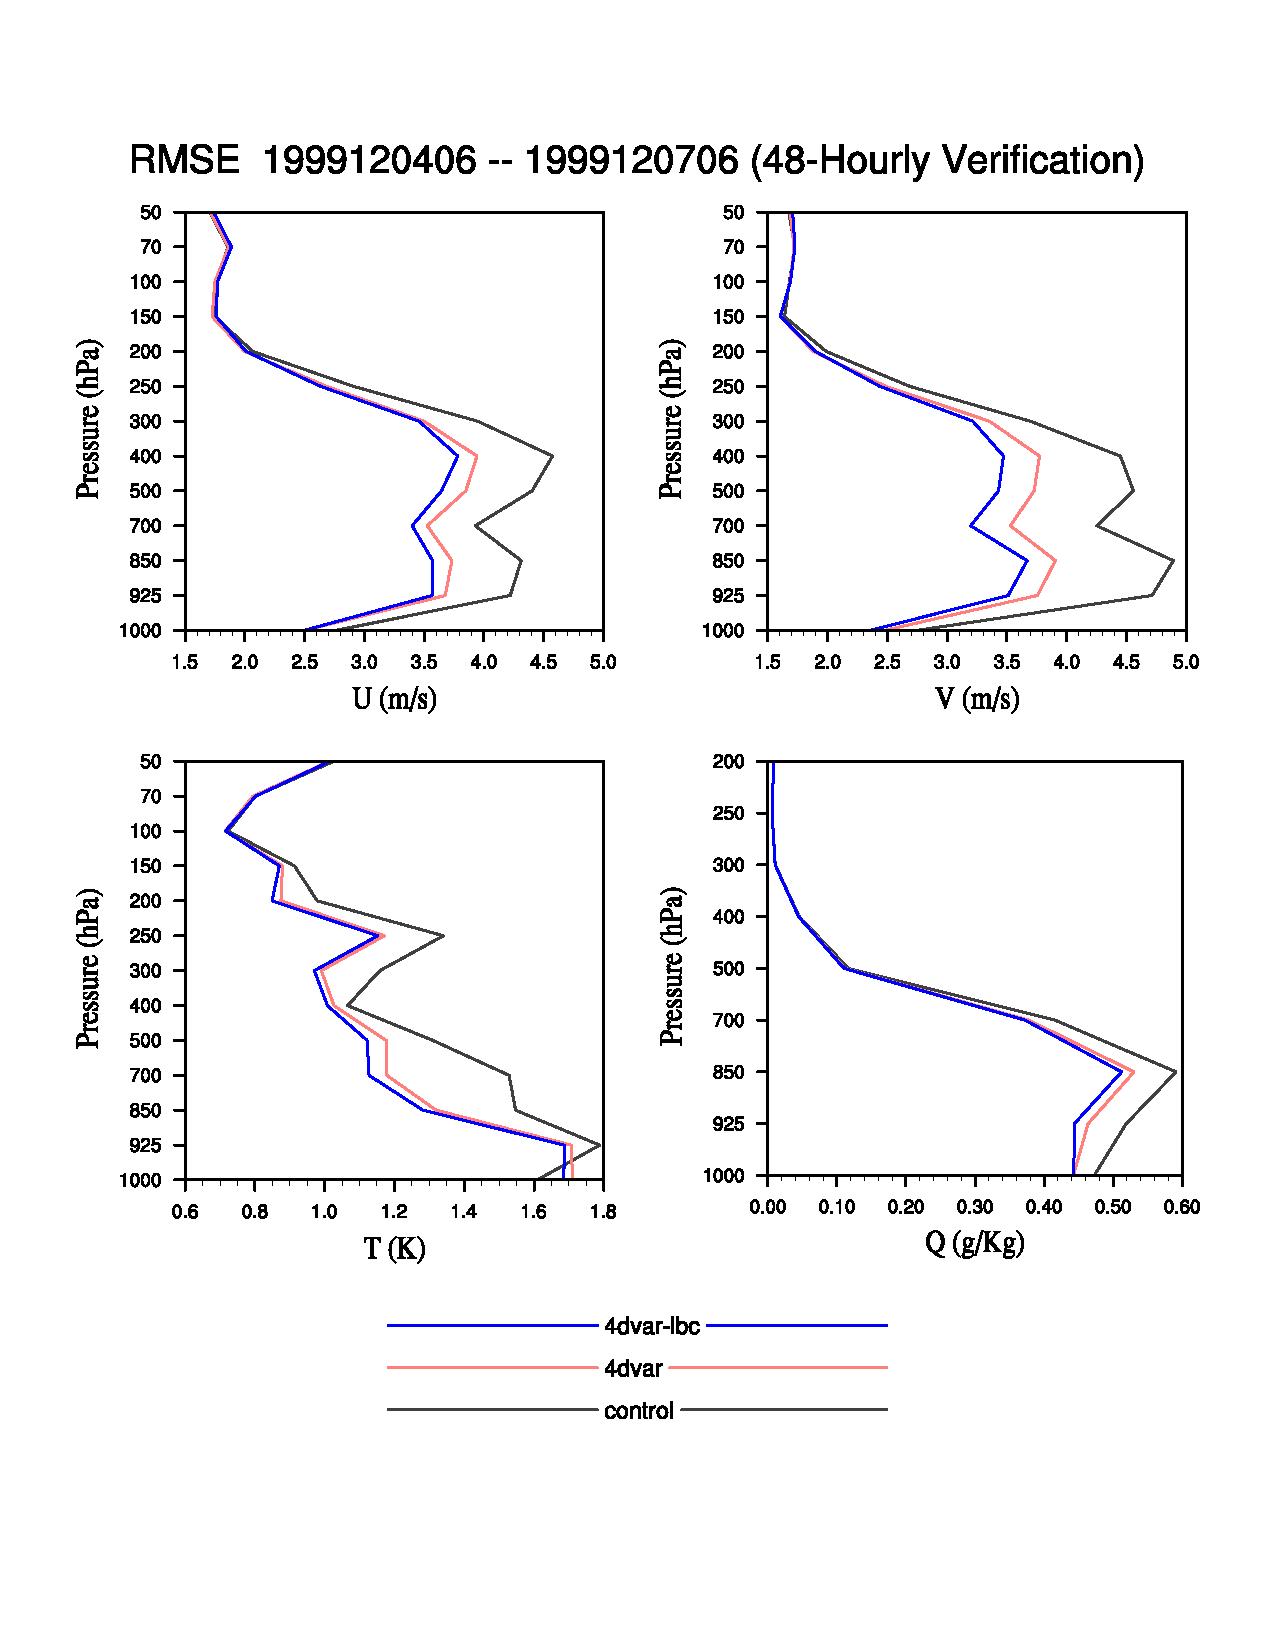
\includegraphics[width=0.5\textwidth]{figures/Profile_RMSE-hr48_lbc.pdf}
        }\\ %  ------- End of the first row ----------------------%
%
    \end{center}
  \caption{RMSE (root mean squre error) verification scores for wind, temperature and moisture forecasts over a Scandinavian domain as verified against ECMWF ERA-40 re-analysis dataset for the forecast lengths +24h and +48h. Verification scores are averaged from the $1^{st}$ to $5^{th}$ of December 1999. Experiments nolbc (red lines), lbc (blue lines) and control run (black lines).}\label{fig:denmark}
\end{figure}

\begin{figure}[t]
 \begin{center}
%
        \subfigure[Observational precipitation (NCEP Stage IV) ]{%
            \label{fig:rainfall_obs}
            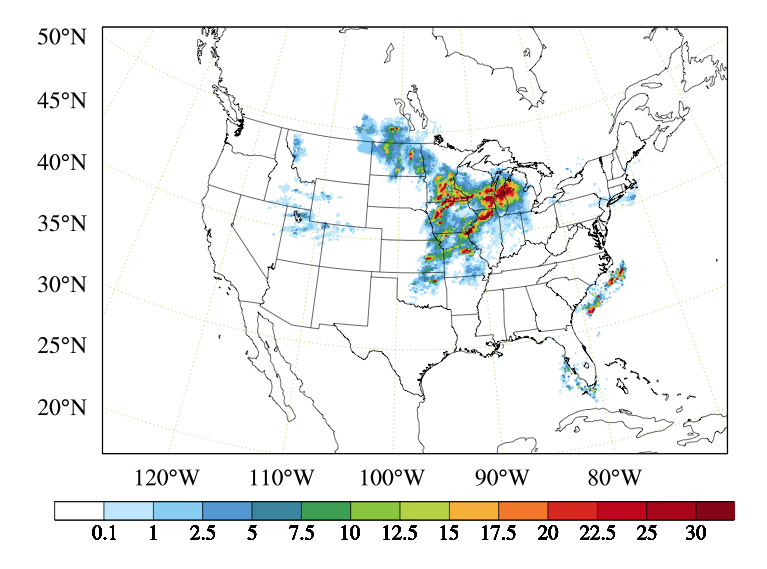
\includegraphics[width=0.5\textwidth]{figures/rainfall_obs.png}
        }%
        \\
        \subfigure[control run]{%
           \label{fig:rainfall_ctl}
           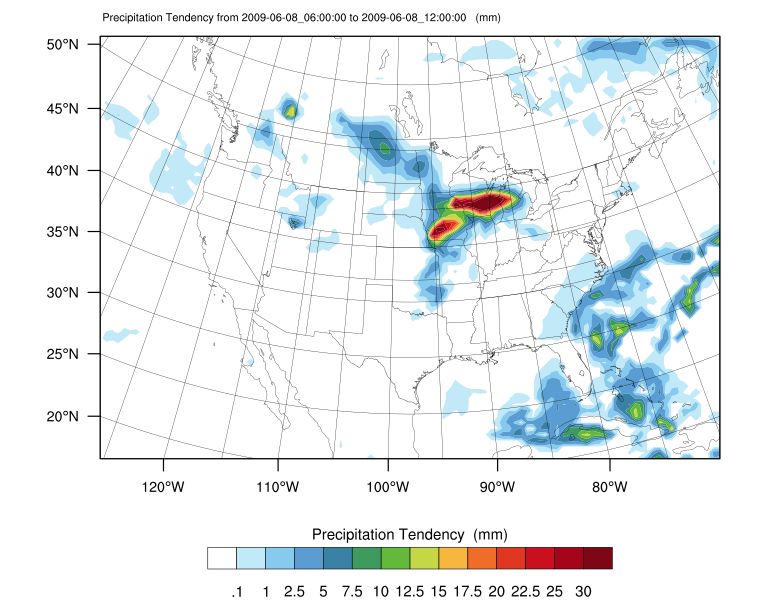
\includegraphics[width=0.5\textwidth]{figures/rainfall_control.png}
        }\\ %  ------- End of the first row ----------------------%
         \subfigure[4dvar run]{%
           \label{fig:rainfal_4dvar}
           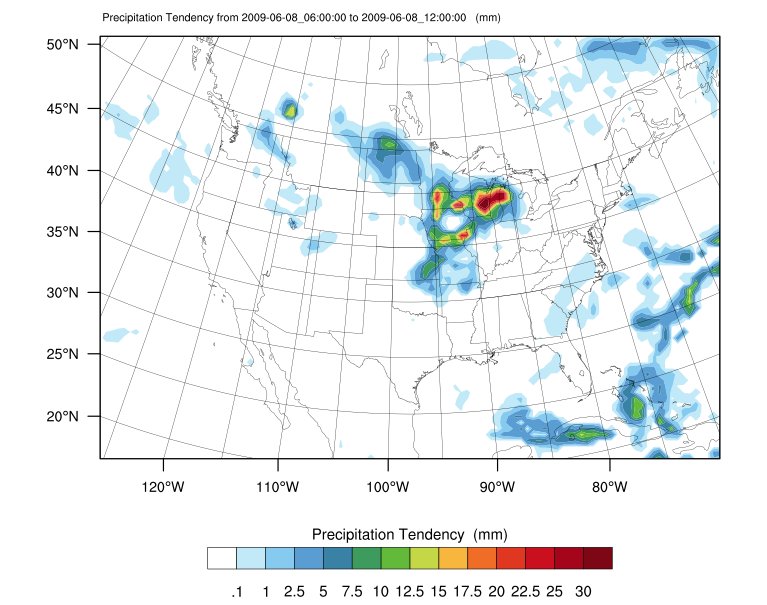
\includegraphics[width=0.5\textwidth]{figures/rainfall_4dvar.png}
        }\\ %  ------- End of the first row ----------------------%
%
 \end{center}
 \caption{0-6h precipitation observation and simulations from 2009060806-2009060812. (a) observational precipitation from NCEP stage IV. (b) control run from FNL. (c) 4D-Var run with assimilation of rainfall data.}\label{fig:rainfall}
\end{figure}

\begin{figure}[t]
 \begin{center}
%
        \subfigure[MPMD]{%
            \label{fig:coupling_mpmd}
            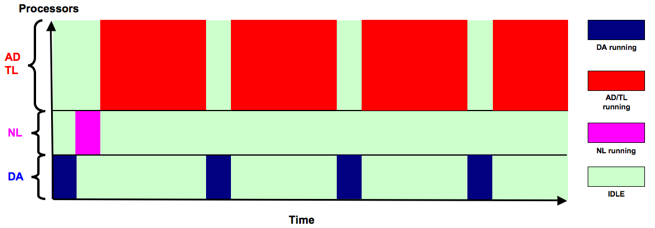
\includegraphics[width=1.0\textwidth]{figures/mpmd_wrf4dvar.png}
        }%
        \\
        \subfigure[SMMD]{%
           \label{fig:coupling_spmd}
           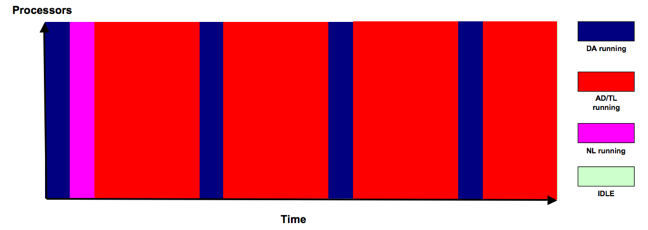
\includegraphics[width=1.0\textwidth]{figures/single_exe_wrf4dvar.png}
        }\\ %  ------- End of the first row ----------------------%
  %
 \end{center}
 \caption{Coupling time axis with MPMD coupling (top) and SPMD coupling (bottom).}\label{fig:coupling}
\end{figure}


\begin{figure}[t]
  \noindent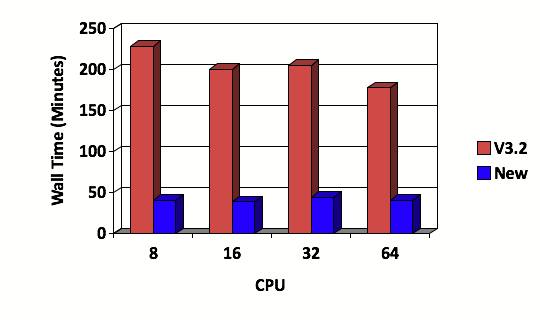
\includegraphics[width=40pc,angle=0]{figures/big_case_performance.png}\\
  \caption{Performance comparison of upgraded single executable WRF 4D-Var and MPMD WRF 4D-Var.}\label{performance}
\end{figure}

\begin{figure}[t]
  \noindent\includegraphics[width=40pc,angle=0]{figures/4dvartime.eps}\\
  \caption{Parallel performance of single executable WRF 4D-Var.}\label{4dvartime}
\end{figure}

\begin{figure}[t]
 \begin{center}
%
        \subfigure[850 hPa ]{%
          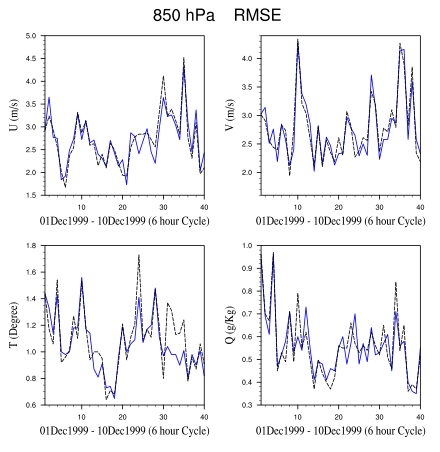
\includegraphics[width=0.5\textwidth]{figures/multi_inc_verif_0_850hpa.png}
        }%
        \\
        \subfigure[500hPa]{%
           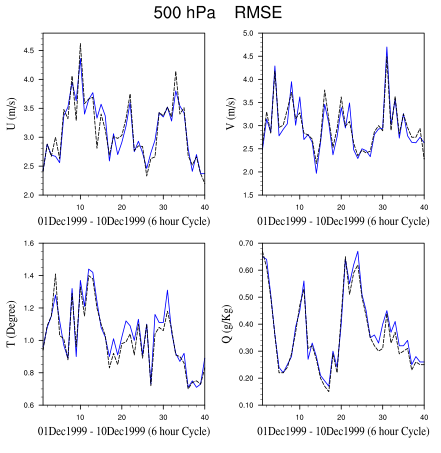
\includegraphics[width=0.5\textwidth]{figures/multi_inc_verif_0_500hpa.png}
        }\\ %  ------- End of the first row ----------------------%
%
 \end{center}
 \caption{Comparison of the 0h analysis verifications of the wind, temperature and moisture between full-resolution and multi-incremental 4D-Var from December 1 to 10, 1999 for Denmark case. (a) 850 hPa. (b) 500 hPa. Black dash line is the full-resolution 4D-Var and blue line is for the multi-incremental 4D-Var}\label{fig:multi_inc_0h}
\end{figure}

\begin{figure}[t]
 \begin{center}
%
        \subfigure[850 hPa ]{%
          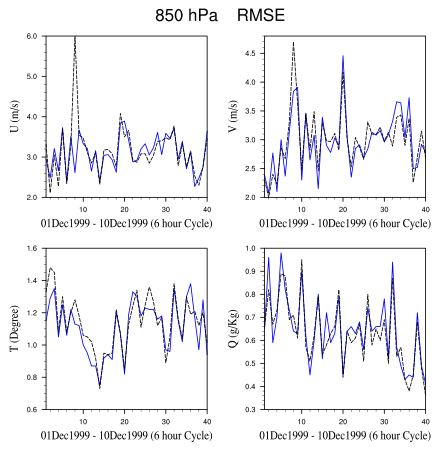
\includegraphics[width=0.5\textwidth]{figures/multi_inc_verif_24_850hpa.png}
        }%
        \\
        \subfigure[500hPa]{%
           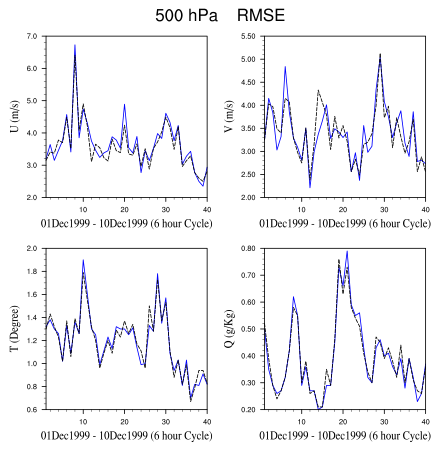
\includegraphics[width=0.5\textwidth]{figures/multi_inc_verif_24_500hpa.png}
        }\\ %  ------- End of the first row ----------------------%
%
 \end{center}
 \caption{Comparison of the 24h forecast verifications of the wind, temperature and moisture between full-resolution and multi-incremental 4D-Var from December 1 to 10, 1999 for Denmark case. (a) 850 hPa. (b) 500 hPa. Black dash line is the full-resolution 4D-Var and blue line is for the multi-incremental 4D-Var}\label{fig:multi_inc_24h}
\end{figure}


%%%%%%%%%%%%%%%%%%%%%%%%%%%%%%%%%%%%%%%%%%%%%%%%%%%%%%%%%%%%%%%%%%%%%
% ACKNOWLEDGMENTS
%%%%%%%%%%%%%%%%%%%%%%%%%%%%%%%%%%%%%%%%%%%%%%%%%%%%%%%%%%%%%%%%%%%%%

\begin{acknowledgment}
The National Center for Atmospheric Research is sponsored by the National
Science Foundation.  This work is supported by the Air Force Weather Agency.
\end{acknowledgment}


%%%%%%%%%%%%%%%%%%%%%%%%%%%%%%%%%%%%%%%%%%%%%%%%%%%%%%%%%%%%%%%%%%%%%
% REFERENCES
%%%%%%%%%%%%%%%%%%%%%%%%%%%%%%%%%%%%%%%%%%%%%%%%%%%%%%%%%%%%%%%%%%%%%
% Create a bibliography directory and place your .bib file there.
\ifthenelse{\boolean{dc}}
{}
{\clearpage}
\bibliographystyle{ametsoc}
\bibliography{../bibliography/references}

\end{document}
%%%%%%%%%%%%%%%%%%%%%%%%%%%%%%%%%%%%%%%%%%%%%%%%%%%%%%%%%%%%%%%%%%%%%
% END OF TEMPLATE
%%%%%%%%%%%%%%%%%%%%%%%%%%%%%%%%%%%%%%%%%%%%%%%%%%%%%%%%%%%%%%%%%%%%%
